%% Copernicus Publications Manuscript Preparation Template for LaTeX Submissions
%% ---------------------------------
%% This template should be used for copernicus.cls
%% The class file and some style files are bundled in the Copernicus Latex Package, which can be downloaded from the different journal webpages.
%% For further assistance please contact Copernicus Publications at: production@copernicus.org
%% https://publications.copernicus.org/for_authors/manuscript_preparation.html

%% Please use the following documentclass and journal abbreviations for preprints and final revised papers.

%% 2-column papers and preprints
\documentclass[hess, manuscript]{copernicus}

%\usepackage{graphics} % scalebox
\usepackage{booktabs} % toprule, bottomrule

% para los anexos
\usepackage[toc,page]{appendix}

%\renewcommand\appendixpagename{Anexos}

\renewcommand{\appendix}{
  % "Copied" from the \appendix command
  \setcounter{section}{0}
  \setcounter{subsection}{0}
  \renewcommand{\thesection}{\Alph{section}}

  \counterwithin{figure}{section}
  \counterwithin{table}{section}
  \phantomsection
  \addcontentsline{toc}{part}{\appendixname} % Format appendix in TOC like \part

  % Inspired from \part in book class
  \clearpage
  \thispagestyle{plain}
  \vspace*{\fill}
  {\centering
    \normalfont\Huge
  \textbf{Anexos}\par}
  \vfill\newpage
}

%% Journal abbreviations (please use the same for preprints and final revised papers)

% Advances in Geosciences (adgeo)
% Advances in Radio Science (ars)
% Advances in Science and Research (asr)
% Advances in Statistical Climatology, Meteorology and Oceanography (ascmo)
% Aerosol Research (ar)
% Annales Geophysicae (angeo)
% Archives Animal Breeding (aab)
% Atmospheric Chemistry and Physics (acp)
% Atmospheric Measurement Techniques (amt)
% Biogeosciences (bg)
% Climate of the Past (cp)
% DEUQUA Special Publications (deuquasp)
% Earth Surface Dynamics (esurf)
% Earth System Dynamics (esd)
% Earth System Science Data (essd)
% E&G Quaternary Science Journal (egqsj)
% EGUsphere (egusphere) | This is only for EGUsphere preprints submitted without relation to an EGU journal.
% European Journal of Mineralogy (ejm)
% Fossil Record (fr)
% Geochronology (gchron)
% Geographica Helvetica (gh)
% Geoscience Communication (gc)
% Geoscientific Instrumentation, Methods and Data Systems (gi)
% Geoscientific Model Development (gmd)
% History of Geo- and Space Sciences (hgss)
% Hydrology and Earth System Sciences (hess)
% Journal of Bone and Joint Infection (jbji)
% Journal of Micropalaeontology (jm)
% Journal of Sensors and Sensor Systems (jsss)
% Magnetic Resonance (mr)
% Mechanical Sciences (ms)
% Natural Hazards and Earth System Sciences (nhess)
% Nonlinear Processes in Geophysics (npg)
% Ocean Science (os)
% Polarforschung - Journal of the German Society for Polar Research (polf)
% Primate Biology (pb)
% Proceedings of the International Association of Hydrological Sciences (piahs)
% Safety of Nuclear Waste Disposal (sand)
% Scientific Drilling (sd)
% SOIL (soil)
% Solid Earth (se)
% State of the Planet (sp)
% The Cryosphere (tc)
% Weather and Climate Dynamics (wcd)
% Web Ecology (we)
% Wind Energy Science (wes)

%% \usepackage commands included in the copernicus.cls:
%\usepackage[german, english]{babel}
%\usepackage{tabularx}
%\usepackage{cancel}
%\usepackage{multirow}
%\usepackage{supertabular}
%\usepackage{algorithmic}
%\usepackage{algorithm}
%\usepackage{amsthm}
%\usepackage{float}
%\usepackage{subfig}
%\usepackage{rotating}

\begin{document}

\title{"Uso de modelos de aprendizaje automático para la predicción de caudales en el Río Cautín utilizando R" \\
Informe Escrito Proyecto Final}

% \Author[affil]{given_name}{surname}

%\Author[][EMAIL]{}{} %% correspondence author
%\Author[]{}{}

%\affil[]{ADDRESS}

\Author[1][g.sepulveda14@ufromail.cl]{Gadiel}{Sepúlveda Aguilera}
\affil[1]{Curso IIO222, 2025-S1, Equipo 07}

\Author[1]{Rocío}{Cano Manzano}

%% The [] brackets identify the author with the corresponding affiliation. 1, 2, 3, etc. should be inserted.

%% If an author is deceased, please mark the respective author name(s) with a dagger, e.g. "\Author[2,$\dag$]{Anton}{Smith}", and add a further "\affil[$\dag$]{deceased, 1 July 2019}".

%% If authors contributed equally, please mark the respective author names with an asterisk, e.g. "\Author[2,*]{Anton}{Smith}" and "\Author[3,*]{Bradley}{Miller}" and add a further affiliation: "\affil[*]{These authors contributed equally to this work.}".

\runningtitle{TEXT}

\runningauthor{TEXT}

\received{}
\pubdiscuss{} %% only important for two-stage journals
\revised{}
\accepted{}
\published{}

%% These dates will be inserted by Copernicus Publications during the typesetting process.

\firstpage{1}

\maketitle

\begin{abstract}
  River floods have posed an ongoing risk for cities and communities nearby. The Cautín River, on the Araucania Region, Chile, has shown a surge in flood events, affecting particularly vulnerable zones, and future phenomena are expected to cause higher damage due to climate change. Therefore, the devolpment and usage of early warning systems is crucial to reduce their cost and impact. Over the last few years, an increasing amount of resources have been invested on machine learning models for forecasting, which promise accurate results with little computational effort, as research shows. The following work aimed to evaluate the accuracy of river flow forecasting on a single gauge at the Cautín catchment area, based on river flow and precipitation information using three different models: xgboost, LSTM and random forests. The implementation showed that the RandomForest model performed best, giving an NSE of 0.92, followed by xgboost and LSTM. S
\end{abstract}

%\copyrightstatement{TEXT} %% This section is optional and can be used for copyright transfers.

\introduction  %% \introduction[modified heading if necessary]
\label{sec:Introduction}

El río Cautín, ubicado en la región de La Araucanía, nace en la falda sur del volcán Lonquimay y fluye hacia el sureste hasta confluir con el río Chol Chol, dando origen al río Imperial \citep{richard_cerda_respuesta_2014}. Con una longitud aproximada de 174 kilómetros, su curso atraviesa las comunas de Curacautín, Lautaro, Vilcún, Padre Las Casas y Temuco, antes de confluir con el río Quepe, lo que evidencia su relevancia tanto geográfica como social.

Este río tiene un régimen pluvial, lo que significa que se alimenta principalmente de agua de lluvia. Así, han sido frecuentes las crecidas e inundaciones que han impactado considerablemente a las comunidades aledañas, y el cambio climático sólo augura un recrudecimiento en estos fenómenos. Según \citet{padilla_turra_registros_2024}, el SENAPRED ha registrado un total de veintiséis emergencias asociadas a crecidas en el Cautín, destacando en junio del 2018 una que finalmente provocó el desplome parcial de un tramo del puente ferroviario que cruzaba el río. Por otra parte, en 2021, \citet{el_mostrador_intendencia_2021} advirtió sobre una alarma emitida por un riesgo de inundación en Temuco y Padre Las Casas; y, dos años después, \citet{mennickent_barros_desbordes_2023} contó que, por un desborde ocurrido en el sector de Rariruca, que une Curacautín con Lautaro, se emitió alerta amarilla en la primera comuna.

Esta situación es de especial preocupación, considerando que en Temuco, por ejemplo, los barrios asociados a la ribera del Cautín son barrios particularmente vulnerables al haberse desarrollado con escasa planificación. \citep{acuna_munoz_volver_2020}. Por lo tanto, surge la necesidad de contar con medidas que permitan responder adecuadamente a estos desastres. En particular, la implementación de sistemas de alerta temprana permite ahorrar hasta diez veces el costo de implementación en pérdidas materiales y humanas. \citep{global_commission_on_adaptation_adapt_nodate}.

El desarrollo de estrategias de manejo de riesgos sostenibles y eficientes bajo condiciones cambiantes requiere comprender los cambios temporales en las causas y efectos de las inundaciones \citep{kreibich_panta_2023}. Así, especialmente en la cuenca a estudiar, es relevante estudiar la incidencia de las precipitaciones sobre el caudal del río. Por otra parte, el avance de la tecnología ha sido tal que realizar predicciones a grandes escalas se ha hecho posible \citep{arnal_towards_2025}. En cuanto a esta materia, existe toda una rama emergente de investigación, donde existen tanto modelos deterministas como probabilísticos. Estos últimos tienen la ventaja de manejar la incertidumbre inherente a estos fenómenos \citep{wakai_historical_2025}.

Dentro de esta última categoría, en los últimos años se dado un énfasis al desarrollo y evaluación de predicciones mediante aprendizaje automático. Cada modelo tiene sus ventajas y desventajas y su aplicabilidad depende de la tarea a resolver y los datos disponibles \citep{fischer_impact_2025}. Citando un caso notable, \citet{luppichini_machine_2024} estudiaron modelos LSTM sobre una cuenca del noroeste de Italia para predecir alturas hidrométricas en una red de estaciones. Los modelos desarrollados ofrecieron predicciones reproducibles, con un bajo costo computacional y errores de unos pocos centímetros. La única observación es que los modelos presentaron una tendencia a subestimar los valores a medida que aumentaba el tiempo de anticipación.

A la fecha de publicación, el presente trabajo propone un enfoque pionero en la Región de la Araucanía al poner a prueba el rendimiento del aprendizaje automático para sistemas de alerta temprana. El objetivo general de este proyecto fue evaluar la precisión de las predicciones de caudal en una estación fluviométrica para diferentes modelos de aprendizaje automático en base a datos de caudal y precipitaciones. Los objetivos específicos fueron:
\begin{itemize}
  \item Entrenar los modelos de aprendizaje automático xgboost, randomforest y LSTM para obtener proyecciones de caudal en base a datos hidrológicos históricos.
  \item Comparar los niveles de caudal predichos por cada modelo con datos históricos en diferentes momentos del sistema.
  \item Implementar una aplicación web que permita la visualización, análisis y descarga de los resultados obtenidos.
\end{itemize}

%%%%%%%%%%%%%%%%%%%%%%%%%%%%%%%%%%%%%%%%%%%%%%%%%%%%%%%%%%%%%%%%%%
%%%%%%%%%%%%%%%%%%%%%%%%%%%%%%%%%%%%%%%%%%%%%%%%%%%%%%%%%%%%%%%%%%
\section{Metodología}
\label{sec:Metodologia}

\subsection{Datos utilizados}

Se recogieron las variables de precipitaciones y caudal desde los sitios web \url{} y \url{https://snia.mop.gob.cl/BNAConsultas/reportes}, respectivamente. En ambos casos, se recogieron series temporales con inicio el 1 de enero de 2002 y fin el 31 de diciembre de 2024. Las restricciones impuestas por los mencionados portales obligaron a la descarga de los datos por fragmentos, en periodos de 1 año. La frecuencia de los datos es sub-diaria, con abundantes tramos en frecuencia regular horaria. Esta información se resumen en la Tabla \ref{fig:gauges}.

\begin{table}
  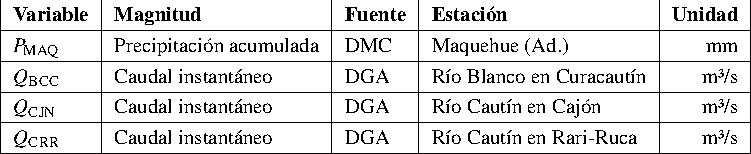
\includegraphics[scale=1]{Tablas_pdf/t01.pdf}
  \caption{Oh}
  \label{fig:gauges}
\end{table}

(nuevo escrito)
La zona estudiada corresponde a la cuenca del Cautín Alto, ubicada en la Región de La Araucanía, Chile. Se utilizaron registros provenientes de tres estaciones fluviométricas dependientes de la Dirección General de Aguas (DGA): Río Cautín en Cajón (06109001-6), Río Cautín en Rari-Ruca (06108001-2) y Río Blanco en Curacautín (06101001-5). La estación objetivo fue Cajón, mientras que las otras dos se utilizaron como entradas al sistema. Adicionalmente, se consideró la estación pluviométrica Maquehue (380005), dependiente de la Dirección Meteorológica de Chile (DMC).

Las variables utilizadas fueron el caudal instantáneo, con unidades en [m³/s], y la precipitación acumulada, en [mm]. Se descargaron series temporales desde los portales oficiales de la DGA (https://snia.mop.gob.cl/BNAConsultas/reportes) y de la DMC (https://climatologia.meteochile.gob.cl). El rango temporal abarcó desde el 1 de enero de 2002 hasta el 31 de diciembre de 2024. Debido a las limitaciones de los portales, fue necesario descargar los datos en fragmentos anuales.

En cuanto a la frecuencia, si bien la información tiene carácter sub-diario, se identificaron numerosos tramos con frecuencia regular horaria, que fueron seleccionados cuidadosamente para el análisis. En el caso de la estación Maquehue, la precipitación se encuentra disponible en intervalos de 6 horas. Para confirmar la zona horaria asociada a las series temporales, se solicitó información formal a la DGA, mediante el código AM001W0186491, confirmando que todos los datos se encuentran en UTC -4.

Un aspecto particular de los archivos de caudal descargados es que se encontraban en formato antiguo .xls (Excel 97-2003), con una estructura poco estandarizada. Cada archivo contiene bloques mensuales de datos organizados horizontalmente, con tres registros paralelos por hoja, lo que dificulta su comprensión y lectura directa. Por lo tanto, se implementó un conjunto de funciones específicas para extraer, limpiar y transformar esta información en un formato útil para el modelamiento.

\subsection{Modelos a evaluar}

Se escogieron tres modelos de aprendzaje automático para esta evaluación. En primer lugar, el modelo xgboost es una implementación del modelo de descenso de grandiente, desarrollado por Cada uno de estos modelos se describe extensivamente en el anexo \ref{appendix:Anexo A}.

En los tres casos, la variable a obtener,
(nuevo escrito)
Con el objetivo de predecir el caudal en la estación Cajón, se evaluaron tres modelos de aprendizaje automático:

XGBoost, un algoritmo de boosting basado en árboles de decisión y descendiente del gradiente.

Random Forest, un ensamble de árboles de regresión que permite capturar relaciones no lineales y reducir el sobreajuste.

LSTM (Long Short-Term Memory), una red neuronal recurrente diseñada para modelar series temporales con dependencias de largo plazo.

En todos los casos, la variable a predecir fue el caudal en la estación Cajón, utilizando como entradas los valores de caudal en Rari-Ruca y Río Blanco, así como la precipitación acumulada en Maquehue. Se consideraron diferentes ventanas de desfase temporal (por ejemplo, 0, 3, 6, 9 y 12 horas) para evaluar la sensibilidad de los modelos ante distintas condiciones hidrológicas.

Una diferencia clave entre el modelo LSTM y los modelos RandomForest y xgboost es que el primero tiene una dependencia temporal explícita, mientras que los siguientes no. De este modo, para comparar los tres modelos, se escogió una ventana temporal fija de $n$ pasos predictivos hacia atrás para obtener una comparación signficativa.

\subsection{Métricas de error}

Se utilizaron dos métricas para analizar el rendimiento de los modelos. Ambos se relacionan con la diferencia entre los valores observados y los valores medidos.

El raíz del error cuadrático medio, abreviado como $\mathrm{RMSE}$ por sus siglas en inglés consiste en la raíz cuadrada de la suma de los cuadrados de las diferencias entre valores estimados y valores medidos. Esta medida ya ha sido usada por \citet{luppichini_machine_2024}, y, considerando un total de $n$ observaciones, se calcula como:

\begin{equation}
  \mathrm{RMSE} = \sqrt{\dfrac{1}{n}\sum_{j=1}^{n} (\hat{Y_i}-Y_i)^2}
\end{equation}

donde $\hat{Y_i}$ representa el valor modelado en el paso de tiempo $i$, mientras que $Y_i$ representa el valor observado en el paso de tiempo $i$.

El Coeficiente de eficiencia de Nash-Sutcliffe, conocido por sus siglas en inglés como NSE, se utiliza para evaluar la eficacia predictiva de un modelo hidrológico. Considerando un total de $n$ observaciones, se calcula como:

\begin{equation}
  \mathrm{NSE} = 1 - \dfrac
  {\sum_{t=1}^n (Q_o^t-Q_m^t)^2}
  {\sum_{t=1}^n (Q_o^t-Q_o)^2}
\end{equation}

donde $Q_o^t$ indica el valor observado al tiempo $t$, $Q_m^t$ indica el valor modelado al tiempo $t$, y $Q_o$ es el promedio de las observaciones. El valor de este coeficiente puede variar entre $-\infty$ y $1$, con $\mathrm{NSE}=1$ siendo el valor óptimo. \citet{melsen_rise_2025} indican que valores entre 0 y 1 se consideran aceptables, mientras que un valor inferior a 1 muestra que el promedio es un mejor predictor que cualquier valor modelado, y, por lo tanto, el modelo no tiene capacidad predictiva.

\subsection{Proceso}
Para llevar a cabo este proyecto, se dividió el flujo de trabajo en cinco grandes etapas: descarga y procesamiento de datos, fusión y partición de datos, entrenamiento de modelos, prueba de modelos, e implementación de la aplicación web.

La primera función se usó para importar los datos. Recibe como entrada una ruta de directorio, donde examina, y, dependiendo del tipo de archivo leído, lee los valores correspondientes.

La segunda función se usó para proesar los datos
%%%%%%%%%%%%%%%%%%%%%%%%%%%%%%%%%%%%%%%%%%%%%%%%%%%%%%%%%%%%%%%%%%
%%%%%%%%%%%%%%%%%%%%%%%%%%%%%%%%%%%%%%%%%%%%%%%%%%%%%%%%%%%%%%%%%%
\section{Resultados}
\label{sec:Resultados}

\subsection{Rendimiento de los modelos}

Una vez entrenados los modelos, se produjeron
\begin{figure}[h]
  \centering
  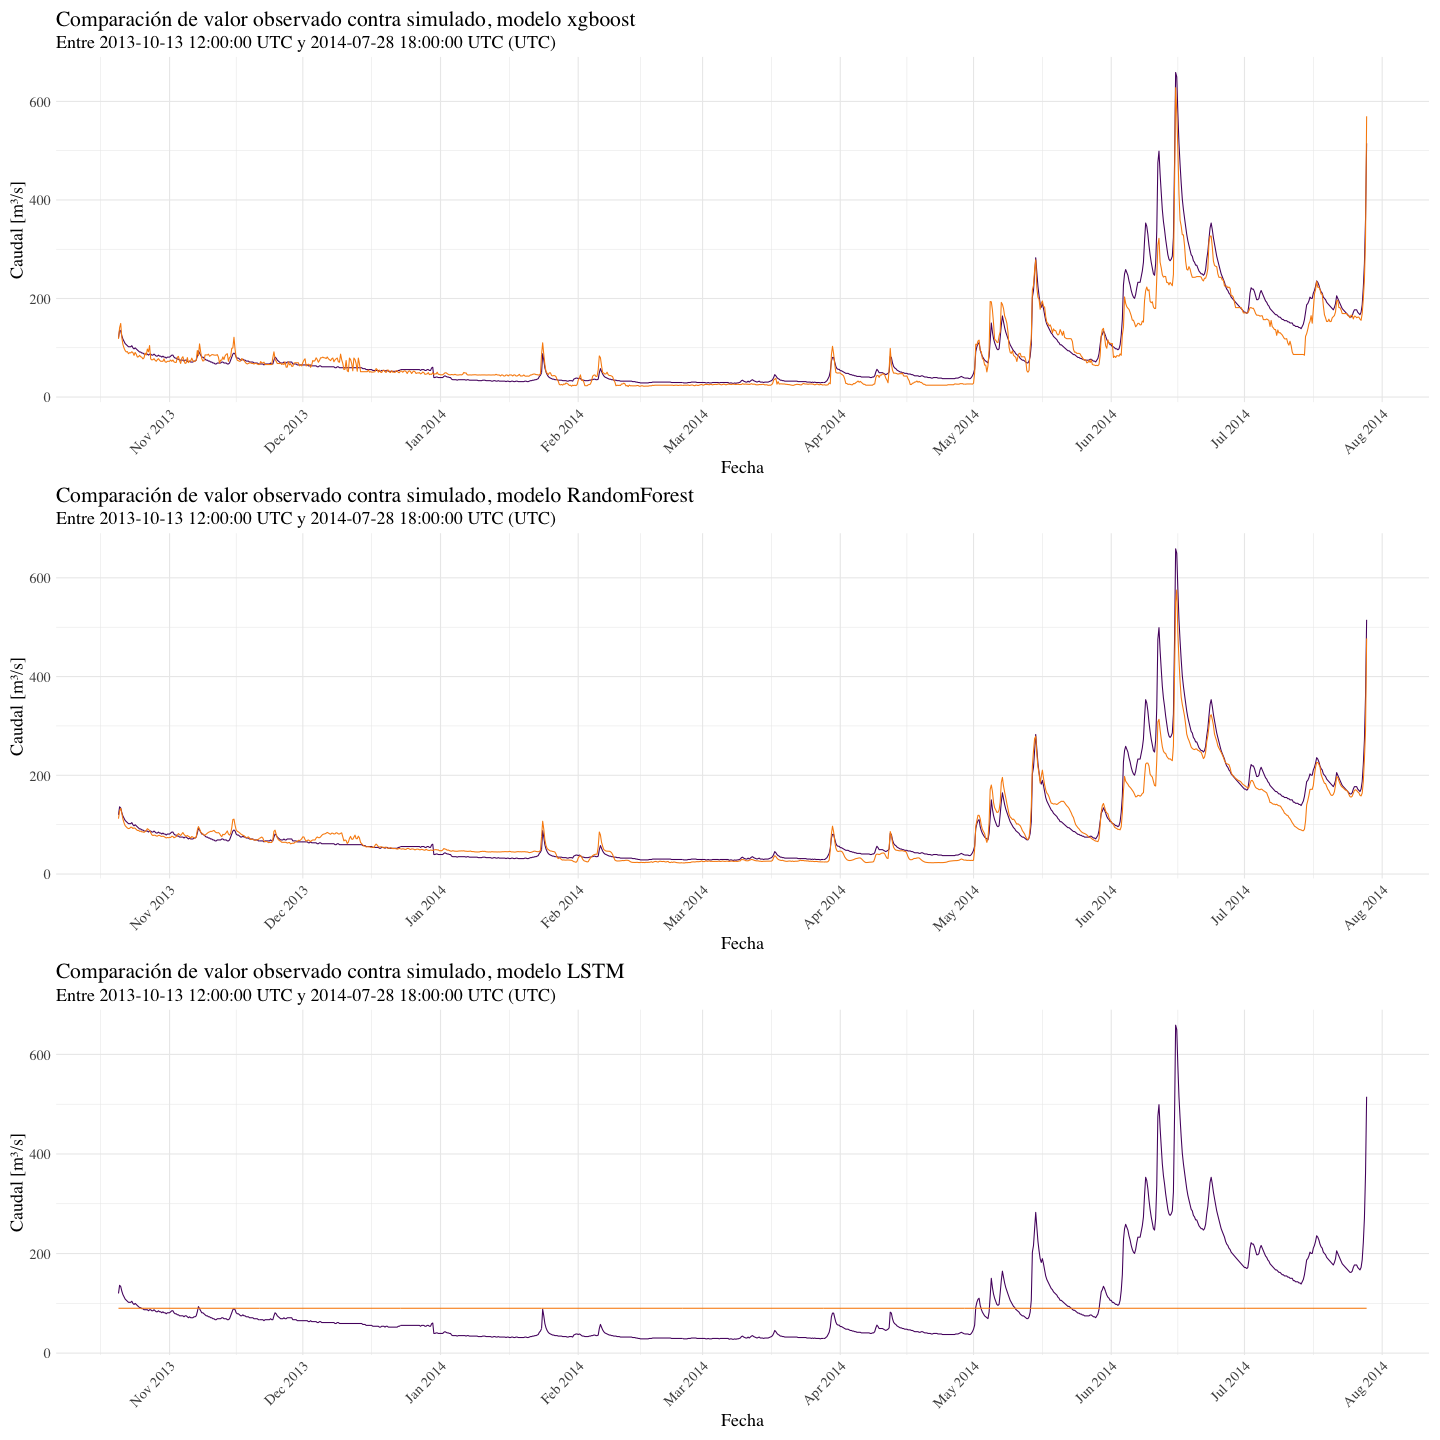
\includegraphics[width=1\textwidth]{Figuras/fig03_comparison.png}
  \caption{Comparación de valores observados y medidos para los tres modelos. En todos los casos, la serie naranja indica los valores simulados, y la serie morada indica los valores observados.}
  \label{fig:example_image}

\end{figure}

%%%%%%%%%%%%%%%%%%%%%%%%%%%%%%%%%%%%%%%%%%%%%%%%%%%%%%%%%%%%%%%%%%
%%%%%%%%%%%%%%%%%%%%%%%%%%%%%%%%%%%%%%%%%%%%%%%%%%%%%%%%%%%%%%%%%%
\section{Discusión}
\label{sec:Discusión}
El presente trabajo buscó traer al contexto local las soluciones en estudio en diferentes partes del mundo, con respecto a

%%%%%%%%%%%%%%%%%%%%%%%%%%%%%%%%%%%%%%%%%%%%%%%%%%%%%%%%%%%%%%%%%%
%%%%%%%%%%%%%%%%%%%%%%%%%%%%%%%%%%%%%%%%%%%%%%%%%%%%%%%%%%%%%%%%%%
\section{Conclusiones}
\label{sec:Conclusiones}

%% The Appendices part is started with the command \appendix;
%% appendix sections are then done as normal sections
\break

%\end{thebibliography}

%% Since the Copernicus LaTeX package includes the BibTeX style file copernicus.bst,
%% authors experienced with BibTeX only have to include the following two lines:
%%
\bibliographystyle{copernicus}
\bibliography{Referencias}

%%
%% URLs and DOIs can be entered in your BibTeX file as:
%%
%% URL = {http://www.xyz.org/~jones/idx_g.htm}
%% DOI = {10.5194/xyz}

%% LITERATURE CITATIONS
%%
%% command                        & example result
%% \citet{jones90}|               & Jones et al. (1990)
%% \citep{jones90}|               & (Jones et al., 1990)
%% \citep{jones90,jones93}|       & (Jones et al., 1990, 1993)
%% \citep[p.~32]{jones90}|        & (Jones et al., 1990, p.~32)
%% \citep[e.g.,][]{jones90}|      & (e.g., Jones et al., 1990)
%% \citep[e.g.,][p.~32]{jones90}| & (e.g., Jones et al., 1990, p.~32)
%% \citeauthor{jones90}|          & Jones et al.
%% \citeyear{jones90}|            & 1990

%% FIGURES

%% When figures and tables are placed at the end of the MS (article in one-column style), please add \clearpage
%% between bibliography and first table and/or figure as well as between each table and/or figure.

% The figure files should be labelled correctly with Arabic numerals (e.g. fig01.jpg, fig02.png).

%% ONE-COLUMN FIGURES

%%f
%\begin{figure}[t]
%\includegraphics[width=8.3cm]{FILE NAME}
%\caption{TEXT}
%\end{figure}
%
%%% TWO-COLUMN FIGURES
%
%%f
%\begin{figure*}[t]
%\includegraphics[width=12cm]{FILE NAME}
%\caption{TEXT}
%\end{figure*}
%
%
%%% TABLES
%%%
%%% The different columns must be seperated with a & command and should
%%% end with \\ to identify the column brake.
%
%%% ONE-COLUMN TABLE
%
%%t
%\begin{table}[t]
%\caption{TEXT}
%\begin{tabular}{column = lcr}
%\tophline
%
%\middlehline
%
%\bottomhline
%\end{tabular}
%\belowtable{} % Table Footnotes
%\end{table}
%
%%% TWO-COLUMN TABLE
%
%%t
%\begin{table*}[t]
%\caption{TEXT}
%\begin{tabular}{column = lcr}
%\tophline
%
%\middlehline
%
%\bottomhline
%\end{tabular}
%\belowtable{} % Table Footnotes
%\end{table*}
%
%%% LANDSCAPE TABLE
%
%%t
%\begin{sidewaystable*}[t]
%\caption{TEXT}
%\begin{tabular}{column = lcr}
%\tophline
%
%\middlehline
%
%\bottomhline
%\end{tabular}
%\belowtable{} % Table Footnotes
%\end{sidewaystable*}
%
%
%%% MATHEMATICAL EXPRESSIONS
%
%%% All papers typeset by Copernicus Publications follow the math typesetting regulations
%%% given by the IUPAC Green Book (IUPAC: Quantities, Units and Symbols in Physical Chemistry,
%%% 2nd Edn., Blackwell Science, available at: http://old.iupac.org/publications/books/gbook/green_book_2ed.pdf, 1993).
%%%
%%% Physical quantities/variables are typeset in italic font (t for time, T for Temperature)
%%% Indices which are not defined are typeset in italic font (x, y, z, a, b, c)
%%% Items/objects which are defined are typeset in roman font (Car A, Car B)
%%% Descriptions/specifications which are defined by itself are typeset in roman font (abs, rel, ref, tot, net, ice)
%%% Abbreviations from 2 letters are typeset in roman font (RH, LAI)
%%% Vectors are identified in bold italic font using \vec{x}
%%% Matrices are identified in bold roman font
%%% Multiplication signs are typeset using the LaTeX commands \times (for vector products, grids, and exponential notations) or \cdot
%%% The character * should not be applied as mutliplication sign
%
%
%%% EQUATIONS
%
%%% Single-row equation
%
%\begin{equation}
%
%\end{equation}
%
%%% Multiline equation
%
%\begin{align}
%& 3 + 5 = 8\\
%& 3 + 5 = 8\\
%& 3 + 5 = 8
%\end{align}
%
%
%%% MATRICES
%
%\begin{matrix}
%x & y & z\\
%x & y & z\\
%x & y & z\\
%\end{matrix}
%
%
%%% ALGORITHM
%
%\begin{algorithm}
%\caption{...}
%\label{a1}
%\begin{algorithmic}
%...
%\end{algorithmic}
%\end{algorithm}
%
%
%%% CHEMICAL FORMULAS AND REACTIONS
%
%%% For formulas embedded in the text, please use \chem{}
%
%%% The reaction environment creates labels including the letter R, i.e. (R1), (R2), etc.
%
%\begin{reaction}
%%% \rightarrow should be used for normal (one-way) chemical reactions
%%% \rightleftharpoons should be used for equilibria
%%% \leftrightarrow should be used for resonance structures
%\end{reaction}
%
%
%%% PHYSICAL UNITS
%%%
%%% Please use \unit{} and apply the exponential notation

%%%%%%%%%%%%%%%%%%%%%%%%%%%%%%%%%%%%%%%%%%%%%%%%%%%%%%%%%%%%%%%%%%
%%%%%%%%%%%%%%%%%%%%%%%%%%%%%%%%%%%%%%%%%%%%%%%%%%%%%%%%%%%%%%%%%%
%\clearpage
\appendix
%\begin{appendices}

%%%%%%%%%%%%%%%%%%%%%%%%%%%%%%%%%%%%%%%%%%%%%%%%%%%%%%%%%%%%%%%%%%
\clearpage
\section{Anexo A: descripción de todas las funciones}
En este anexo se describe...

Metodología
Descarga manual:
Los datos utilizados en esta investigación fueron obtenidos de las fuentes oficiales de información hidrometeorológica en Chile, abarcando el período desde 2002 hasta 2024. Específicamente, los datos horarios de caudal para las estaciones "Río Cautín en Cajón", "Río Cautín en Rari-Ruca" y "Río Blanco" se descargaron directamente desde el sitio web de la Dirección General de Aguas (DGA).

En cuanto a los datos de precipitación de la estación "Maquehue", inicialmente se consultó el sitio web de la Dirección Meteorológica de Chile (DMC). Sin embargo, se constató que la resolución temporal disponible era de seis horas. Con el objetivo de obtener una resolución horaria, se contactó directamente a la DMC vía correo electrónico. Lamentablemente, se confirmó que la única resolución horaria disponible para esta estación era cada seis horas, por lo que se procedió a descargar los datos con la resolución disponible en el sitio web oficial.
Importación de datos:
Una vez obtenidos los datos, se procedió a su importación y manipulación en el entorno de R. Los datos de caudal fueron descargados anualmente en formato .xls, por lo que se leyó cada archivo correspondiente a su año. En contraste, para los datos de precipitaciones, que estaban en formato .csv, solo fue necesario leer un único archivo. Posteriormente, ambos conjuntos de datos fueron reestructurados.
Re-shaping de datos:
La reestructuración de los datos fue un paso crítico debido a las particularidades de los formatos de origen. Los datos de caudal, que se descargaron anualmente y estaban en formato .xls, presentaban una estructura compleja. Cada archivo se dividía por meses, y dentro de cada mes, se encontraban tres bloques repetidos con las columnas "Día", Hora", "Altura (m)", "Caudal (m³/s)", "I" y "O". La lectura de estos datos se realizaba de izquierda a derecha y de arriba hacia abajo, lo que demandó el uso de varias funcione para su correcto ordenamiento y para seleccionar solo las columnas de interés:

D_YMDetect: Esta función detectó filas específicas en el data frame de caudal que contenían únicamente información de mes y año en su tercera columna. Utilizó una expresión regular para identificar el formato “mes/año” (ej., “12/2023”) y devolvió una lista con los índices de estas filas, junto con un desglose de mes y año en columnas separadas.

D_YMAppend: Agregó las columnas de mes (M) y año (Y) a cada data frame de caudal, utilizando la información detectada previamente por D_YMDetect. Los valores de mes y año se asignaron solo en las filas correspondientes, dejando NA en las demás.

D_ColStack: Diseñada para procesar datos hidrométricos anuales de la DGA, esta función apiló la información de los diferentes bloques de columnas en un único data frame ordenado. Asignó siglas identificadoras para caudal y origen según el nombre de la estación, añadió columnas de mes y año, extrajo bloques con datos de día, hora, caudal y origen, y los combinó. Además, limpió y transformó los datos, propagó la información faltante de mes y año, convirtió las columnas a tipos de datos adecuados y generó una columna de fecha completa con zona horaria UTC. El resultado fue un data frame con fecha, caudal y fuente, listo para análisis.

D_JoinByGauge: Procesó una lista de data frames, donde cada uno correspondía a un año de datos de una estación hidrométrica. Aplicó la función D_ColStack a cada data frame y luego unió todos los resultados en un único data frame consolidado para toda la serie temporal de una estación.

D_ProcessAll: Automatizó el procesamiento de datos hidrométricos para todas las estaciones en una lista. Para cada estación, aplicó la función D_JoinByGauge para consolidar y formatear los datos anuales. Finalmente, devolvió una lista con los datos procesados y unidos para cada estación, facilitando el manejo conjunto de múltiples series de tiempo.

Dado que los datos de caudal se encontraban en una resolución horaria, mientras que los datos de precipitación estaban disponibles cada seis horas, fue necesario homogeneizar la resolución temporal de los datos de caudal para que coincidieran con la de los datos pluviométricos. Para lograr esta armonización, se emplearon las siguientes funciones R personalizadas:

TSMerge: Esta función se utilizó para combinar múltiples series temporales provenientes de una lista de data frames, donde cada uno representaba los datos de una estación y compartía una columna común denominada Fecha. La función realizó un merge iterativo de los data frames por la columna Fecha, asegurando que todos los registros fueran mantenidos (utilizando all = TRUE), incluso si no todas las estaciones tenían datos para cada fecha. Finalmente, se verificó que todas las fechas estuvieran en la zona horaria UTC y el resultado se devolvió como un tibble.

TSFilter: Esta función se encargó de filtrar el data frame de series temporales. Su propósito fue conservar únicamente aquellos registros cuya hora fuera un múltiplo de seis (es decir, 00:00, 06:00, 12:00 o 18:00) y cuyos minutos fueran exactamente cero. Este paso fue crucial para reducir los datos de caudal a un paso temporal regular de 6 horas, alineándose con la resolución de las precipitaciones.

TSMergeAndFilter: Esta función combinó las funcionalidades de las dos anteriores. Primero, unió los data frames de la lista de estaciones por la columna Fecha utilizando TSMerge, manteniendo todas las fechas disponibles. Posteriormente, aplicó TSFilter para conservar solo los registros tomados cada 6 horas exactas. El resultado fue un data frame consolidado y con una resolución temporal uniforme de 6 horas, listo para el análisis conjunto de caudal y precipitación.

Una vez aplicadas estas funciones, los datos de caudal quedaron completamente preparados para su utilización en los análisis posteriores.

En contraste, los datos de precipitación, al estar en formato .csv y presentar un diseño más sencillo, solo requirieron de algunas funciones para su correcto ordenamiento, las funciones utilizadas para su procesamiento fueron:

P_Conversion: Procesó un data frame de datos de precipitación, asignando una sigla identificadora según el nombre de la estación. Creó una nueva columna con esta sigla que contenía los valores numéricos de precipitación (RRR6_Valor). Además, convirtió la columna de fecha y hora (momento) en un objeto de fecha con zona horaria definida (tz), y retornó un data frame con la fecha (Fecha) y la precipitación (con nombre dinámico).

P_DateCut: Recortó un data frame de series temporales para incluir solo las filas cuya columna 'Fecha' estuviera dentro de un rango específico. Convirtió las fechas de entrada (formato día-mes-año hora:minuto-segundo) a objetos de fecha-hora y filtró el data frame en consecuencia.

P_ProcessAll: Automatizó el procesamiento de datos de precipitación para una lista de estaciones. Para cada estación, aplicó primero P_Conversion y luego P_DateCut para recortar el rango de fechas según un intervalo dado. Finalmente, devolvió una nueva lista con los datos de precipitación procesados y filtrados para todas las estaciones a partir del 1 de enero de 2002.
Análisis exploratorio de datos:
Una vez que los datos estuvieron limpios y reestructurados, se realizó un Análisis Exploratorio de Datos (AED) para comprender sus características principales y visualizar sus patrones. Para ello, se emplearon las siguientes funciones:

StatSummary: Esta función calculó estadísticas descriptivas básicas (mínimo, cuartiles, mediana, máximo y promedio) para vectores numéricos. Permitió obtener un resumen rápido de la distribución de las variables clave, como el caudal y las precipitaciones.

CategoryCount: Se utilizó para contar la frecuencia de cada categoría en vectores de tipo factor. Esto fue útil para entender la distribución de variables categóricas, si las hubiera, aunque en este caso se aplicó principalmente para validar estructuras de datos.

GlobalSummary: Esta función consolidó un resumen completo de cada data frame, distinguiendo entre columnas numéricas y categóricas. Para las numéricas, aplicó StatSummary, mientras que para las categóricas, usó CategoryCount. El resultado fue una lista con dos elementos: uno para variables numéricas (Num) y otro para categóricas (Cat), proporcionando una visión general de todo el conjunto de datos.

TSBasicPlot: Se empleó para generar gráficos de línea de series temporales. Visualizó la evolución de variables numéricas (como caudal y precipitación) a lo largo del tiempo, utilizando la columna 'Fecha' como eje X. Esta función fue clave para identificar tendencias, estacionalidades y posibles anomalías en los datos.

IntervalComparison: Esta función automatizó la creación de gráficos en archivos PDF para comparar visualmente múltiples variables de series temporales entre diferentes data frames. Para cada data frame de una lista (db), generó un PDF con dos gráficos apilados (layout 2x1) que mostraban la evolución de las variables especificadas, usando colores personalizados. Esta herramienta facilitó la comparación de los patrones de caudal y precipitación entre las distintas estaciones y períodos.

Estas funciones permitieron obtener una comprensión profunda de la distribución, el comportamiento temporal y las interrelaciones de los datos de caudal y precipitación antes de proceder con análisis más complejos.
Selección de intervalos regulares:
Una vez que los datos fueron reestructurados y preparados, el siguiente paso fue seleccionar intervalos regulares para obtener series de datos limpias y consistentes, adecuadas para los modelos que se utilizarían. Para lograr esto, se emplearon las siguientes funciones:

IntervalFind: Esta función identificó y segmentó los data frames de series temporales en intervalos regulares. Calculó la diferencia en minutos entre observaciones consecutivas y agrupó los datos en segmentos continuos donde estas diferencias no superaban un umbral definido (por defecto, 6 minutos). Esto permitió dividir los datos en periodos consistentes sin grandes saltos temporales, devolviendo una lista con estos intervalos como data frames separados.

IntervalFilter: Se utilizó para filtrar la lista de data frames generada por IntervalFind. Esta función eliminó aquellos intervalos que contenían menos filas que un umbral predefinido (por defecto, 100 observaciones). De esta manera, se conservaron solo los intervalos con suficientes datos para asegurar la confiabilidad de los análisis posteriores, contribuyendo a la depuración y calidad del conjunto de datos segmentado.
Entrenamiento de modelos:
Con los datos ya limpios y estructurados, se procedió al entrenamiento de los modelos predictivos. Se utilizaron dos enfoques principales: Random Forest para predicción de caudal con diferentes horizontes y LSTM para modelar la dinámica temporal de los datos.

Modelo Random Forest
Para la predicción del caudal en la estación CJN_Q, se empleó un modelo Random Forest con horizontes predictivos que van desde 1 hasta 6 pasos hacia adelante. La preparación de los datos para este modelo se realizó de la siguiente manera:

Se utilizó el primer intervalo de datos continuos (intervals[[1]]) como conjunto de entrenamiento y el tercer intervalo (intervals[[3]]) como conjunto de validación.

Para cada horizonte de predicción h (donde h=1,…,6), se creó un nuevo conjunto de entrenamiento. La variable objetivo para cada modelo fue el caudal de CJN_Q observado h pasos hacia adelante (lead(CJN_Q, h)).

Las variables predictoras incluyeron los caudales de las estaciones CRR_Q y BCC_Q, así como la precipitación en MAQ_P.

Se entrenó un modelo Random Forest independiente para cada horizonte predictivo (un total de 6 modelos), configurando cada uno con 500 árboles.

Finalmente, cada modelo fue evaluado sobre el conjunto de validación. Las predicciones generadas se compararon visualmente con la serie observada mediante gráficos que se guardaron en formato PNG, lo que permitió una rápida evaluación del rendimiento.

Modelo LSTM (Long Short-Term Memory)
Para predecir el caudal del río en CJN_Q a partir de las variables predictoras (precipitación en MAQ_P y caudales en BCC_Q y CRR_Q), se implementó una red LSTM, ideal para modelar secuencias temporales:

Transformación de Datos: Los datos se transformaron en tensores secuenciales utilizando la clase DataTensorGen. Esta clase es crucial para preparar las entradas del LSTM, creando muestras con una ventana de tiempo de n_steps pasos hacia atrás para predecir un valor futuro. Se generaron tensores separados para los conjuntos de entrenamiento, validación y prueba.

Definición del Modelo: Se definió un modelo LSTM personalizado (LSTMModelGen) que incluyó múltiples capas ocultas y una opción de dropout para prevenir el sobreajuste.

Entrenamiento: El entrenamiento se llevó a cabo con la función luz::fit, utilizando el error cuadrático medio (MSE) como función de pérdida y el optimizador Adam. El proceso se ejecutó por hasta 200 épocas, incorporando parada temprana para evitar el sobreentrenamiento y un ajuste dinámico de la tasa de aprendizaje mediante la estrategia one cycle learning rate.

Predicción: Una vez entrenado, el modelo se utilizó para realizar predicciones sobre el conjunto de prueba. La salida resultante incluye n_steps valores iniciales como NA para asegurar la correcta alineación temporal de las predicciones con los datos observados. Esta arquitectura permitió capturar la compleja dinámica temporal de los datos y anticipar el comportamiento del caudal en función de las variables hidrometeorológicas pasadas.
Prueba de modelos:

Cálculo de métricas de error:
Para evaluar el rendimiento de los modelos predictivos, se utilizaron las métricas Nash-Sutcliffe Efficiency (NSE) y Root Mean Square Error (RMSE). Estas métricas son comúnmente empleadas en el campo de la hidrología y permiten cuantificar la precisión y fiabilidad de las predicciones.

Nash-Sutcliffe Efficiency (NSE)
El NSE es una métrica fundamental para evaluar la capacidad de un modelo de predicción para simular el comportamiento de una serie de datos observados, en comparación con el simple uso del promedio de las observaciones. Su valor oscila entre −∞ y 1. Un valor de 1 indica una coincidencia perfecta entre las predicciones y las observaciones. Un valor de 0 sugiere que el modelo no mejora el rendimiento de una predicción basada únicamente en la media de los datos observados. Valores negativos indican que el modelo es menos preciso que simplemente usar el promedio de los datos, lo que significa que el modelo no es adecuado. El NSE es particularmente útil porque considera tanto la variabilidad de los datos como la magnitud del error, proporcionando una medida integral de la bondad del ajuste del modelo.

Root Mean Square Error (RMSE)
El RMSE es una medida del error promedio entre los valores predichos por el modelo y los valores reales observados. Se calcula como la raíz cuadrada del promedio de los errores al cuadrado, lo que implica que los errores más grandes tienen un impacto desproporcionadamente mayor en el resultado final. La principal ventaja del RMSE es que se expresa en las mismas unidades que la variable que se está prediciendo (en este caso, caudal o precipitación), lo que facilita su interpretación directa en un contexto práctico. Un RMSE bajo indica una alta precisión en las predicciones del modelo, mientras que un RMSE alto sugiere desviaciones significativas. Dado que penaliza fuertemente los errores grandes, el RMSE es una métrica valiosa para identificar y minimizar desviaciones considerables del modelo.
Implementación de aplicación en Shiny:
Para la visualización interactiva de los resultados del modelo, se desarrolló una aplicación web en Shiny. Esta aplicación está diseñada para facilitar la exploración de las predicciones y métricas de los modelos, presentando una interfaz intuitiva con las siguientes características:

La pantalla principal de la aplicación incluye una barra lateral (sidebar) que permite al usuario seleccionar el modelo de interés. Además, cuenta con un calendario para definir el rango de fechas para las cuales se desean observar las predicciones. Un slider facilita la elección del horizonte de predicción, permitiendo visualizar resultados a 0, 3 o 6 horas. Finalmente, un checkbox ofrece la opción de seleccionar la métrica de evaluación a mostrar, pudiendo ser NSE, RMSE o ambas.

El panel derecho de la interfaz está dedicado a la visualización gráfica de las predicciones. Adicionalmente, se incluyen pestañas que organizan la información de manera detallada: una pestaña muestra una tabla con los datos reales y los valores calculados por el modelo seleccionado, mientras que otra presenta las métricas de evaluación elegidas por el usuario.

%%%%%%%%%%%%%%%%%%%%%%%%%%%%%%%%%%%%%%%%%%%%%%%%%%%%%%%%%%%%%%%%%%
%\clearpage
%\section{Anexo X}
%En este anexo se describe...

%\end{appendices}

\section{Anexo B: aplicación web}
\end{document}
